\documentclass{standalone}
\usepackage[T1]{fontenc}
\usepackage[utf8]{inputenc}
\usepackage[usenames,dvipsnames]{xcolor}
\usepackage{tikz}
\usetikzlibrary{plotmarks}
\usetikzlibrary{shapes,snakes,arrows}
\begin{document}
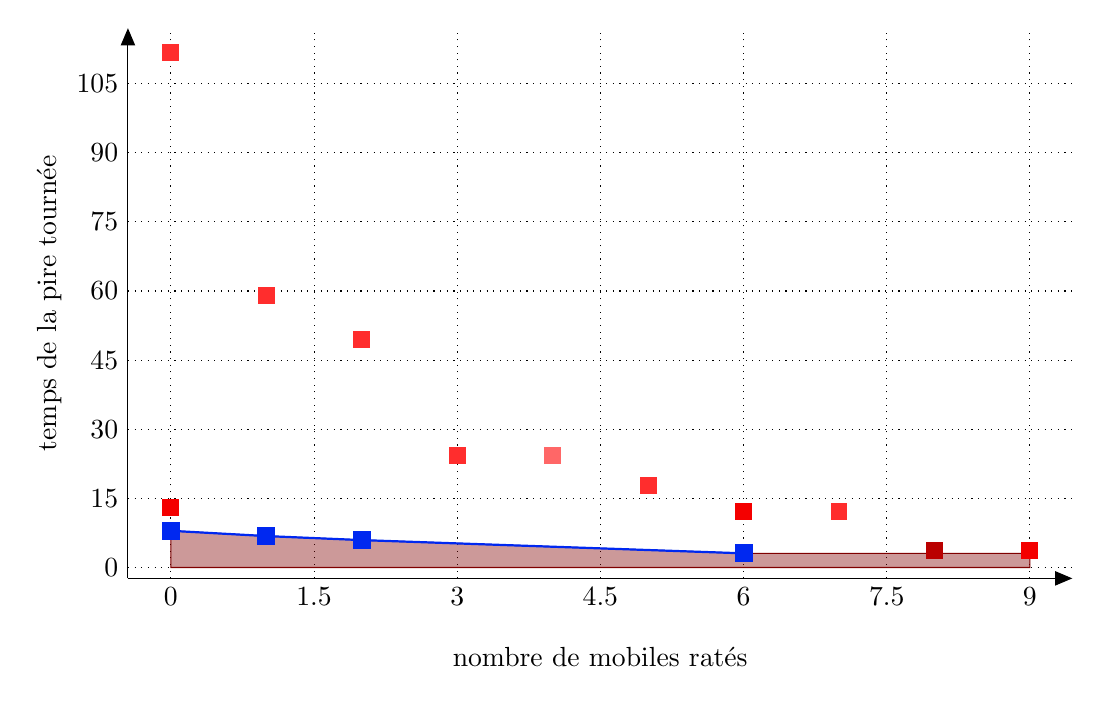
\begin{tikzpicture}[xscale=1.21212,yscale=0.0585229]
\draw[xstep=1.5,ystep=15,thin,dotted,color=Black] (-0.45,-2.35859) grid (9.44446,117.04);
\begin{scope}
  \clip (-0.45,-2.35859) rectangle (9.44446,117.04);
  \definecolor{hvColor}{RGB}{128,0,0}
  \draw[color=hvColor, fill=hvColor, fill opacity=0.4] (0,3.07506) -- (0,7.96854) -- (1,6.82064) -- (2,5.94912) -- (6,3.07506) -| (9,3.07506) |- (0,0) -- cycle;
  \definecolor{pLineColor}{RGB}{186,0,0}
  \definecolor{pPointColor}{RGB}{186,0,0}
  \node[draw,color=pPointColor,fill=pPointColor, inner sep = 0pt, minimum size=2mm] at (0,8.10609) {};
  \node[draw,color=pPointColor,fill=pPointColor, inner sep = 0pt, minimum size=2mm] at (1,7.01988) {};
  \node[draw,color=pPointColor,fill=pPointColor, inner sep = 0pt, minimum size=2mm] at (8,3.63866) {};
  \definecolor{pLineColor}{RGB}{244,0,0}
  \definecolor{pPointColor}{RGB}{244,0,0}
  \node[draw,color=pPointColor,fill=pPointColor, inner sep = 0pt, minimum size=2mm] at (0,13.064) {};
  \node[draw,color=pPointColor,fill=pPointColor, inner sep = 0pt, minimum size=2mm] at (6,12.1234) {};
  \node[draw,color=pPointColor,fill=pPointColor, inner sep = 0pt, minimum size=2mm] at (9,3.63866) {};
  \definecolor{pLineColor}{RGB}{255,45,45}
  \definecolor{pPointColor}{RGB}{255,45,45}
  \node[draw,color=pPointColor,fill=pPointColor, inner sep = 0pt, minimum size=2mm] at (0,111.748) {};
  \node[draw,color=pPointColor,fill=pPointColor, inner sep = 0pt, minimum size=2mm] at (1,59.0744) {};
  \node[draw,color=pPointColor,fill=pPointColor, inner sep = 0pt, minimum size=2mm] at (2,49.4226) {};
  \node[draw,color=pPointColor,fill=pPointColor, inner sep = 0pt, minimum size=2mm] at (3,24.3197) {};
  \node[draw,color=pPointColor,fill=pPointColor, inner sep = 0pt, minimum size=2mm] at (5,17.872) {};
  \node[draw,color=pPointColor,fill=pPointColor, inner sep = 0pt, minimum size=2mm] at (7,12.1234) {};
  \definecolor{pLineColor}{RGB}{255,103,103}
  \definecolor{pPointColor}{RGB}{255,103,103}
  \node[draw,color=pPointColor,fill=pPointColor, inner sep = 0pt, minimum size=2mm] at (4,24.3197) {};
  \definecolor{pLineColor}{RGB}{128,0,0}
  \definecolor{pPointColor}{RGB}{0,40,240}
  \draw[thick,color=pPointColor] (0,7.96854) node[draw,color=pPointColor,fill=pPointColor, inner sep = 0pt, minimum size=2mm] {} -- (1,6.82064) node[draw,color=pPointColor,fill=pPointColor, inner sep = 0pt, minimum size=2mm] {} -- (2,5.94912) node[draw,color=pPointColor,fill=pPointColor, inner sep = 0pt, minimum size=2mm] {} -- (6,3.07506) node[draw,color=pPointColor,fill=pPointColor, inner sep = 0pt, minimum size=2mm] {};
\end{scope}
\draw[->,>=triangle 45] (-0.45,-2.35859) -- coordinate (x axis mid) (9.44446,-2.35859);
\node[below=1cm,anchor=center] at (x axis mid) {nombre de mobiles ratés};
\foreach \x in {0,1.5,3,4.5,6,7.5,9}
  \draw (\x,-2.35859) -- (\x,-2.35859) node[anchor=north] {\x};
\draw[->,>=triangle 45] (-0.45,-2.35859) -- coordinate (y axis mid) (-0.45,117.04);
\node[left=1cm,rotate=90,anchor=center] at (y axis mid) {temps de la pire tournée};
\foreach \y in {0,15,30,45,60,75,90,105}
  \draw (-0.45,\y) -- (-0.45,\y) node[anchor=east] {\y};
\end{tikzpicture}
\end{document}
